\section{Methods}

\subsection{Angle-scanned phase illumination}

\begin{figure}[htbp]
\centering
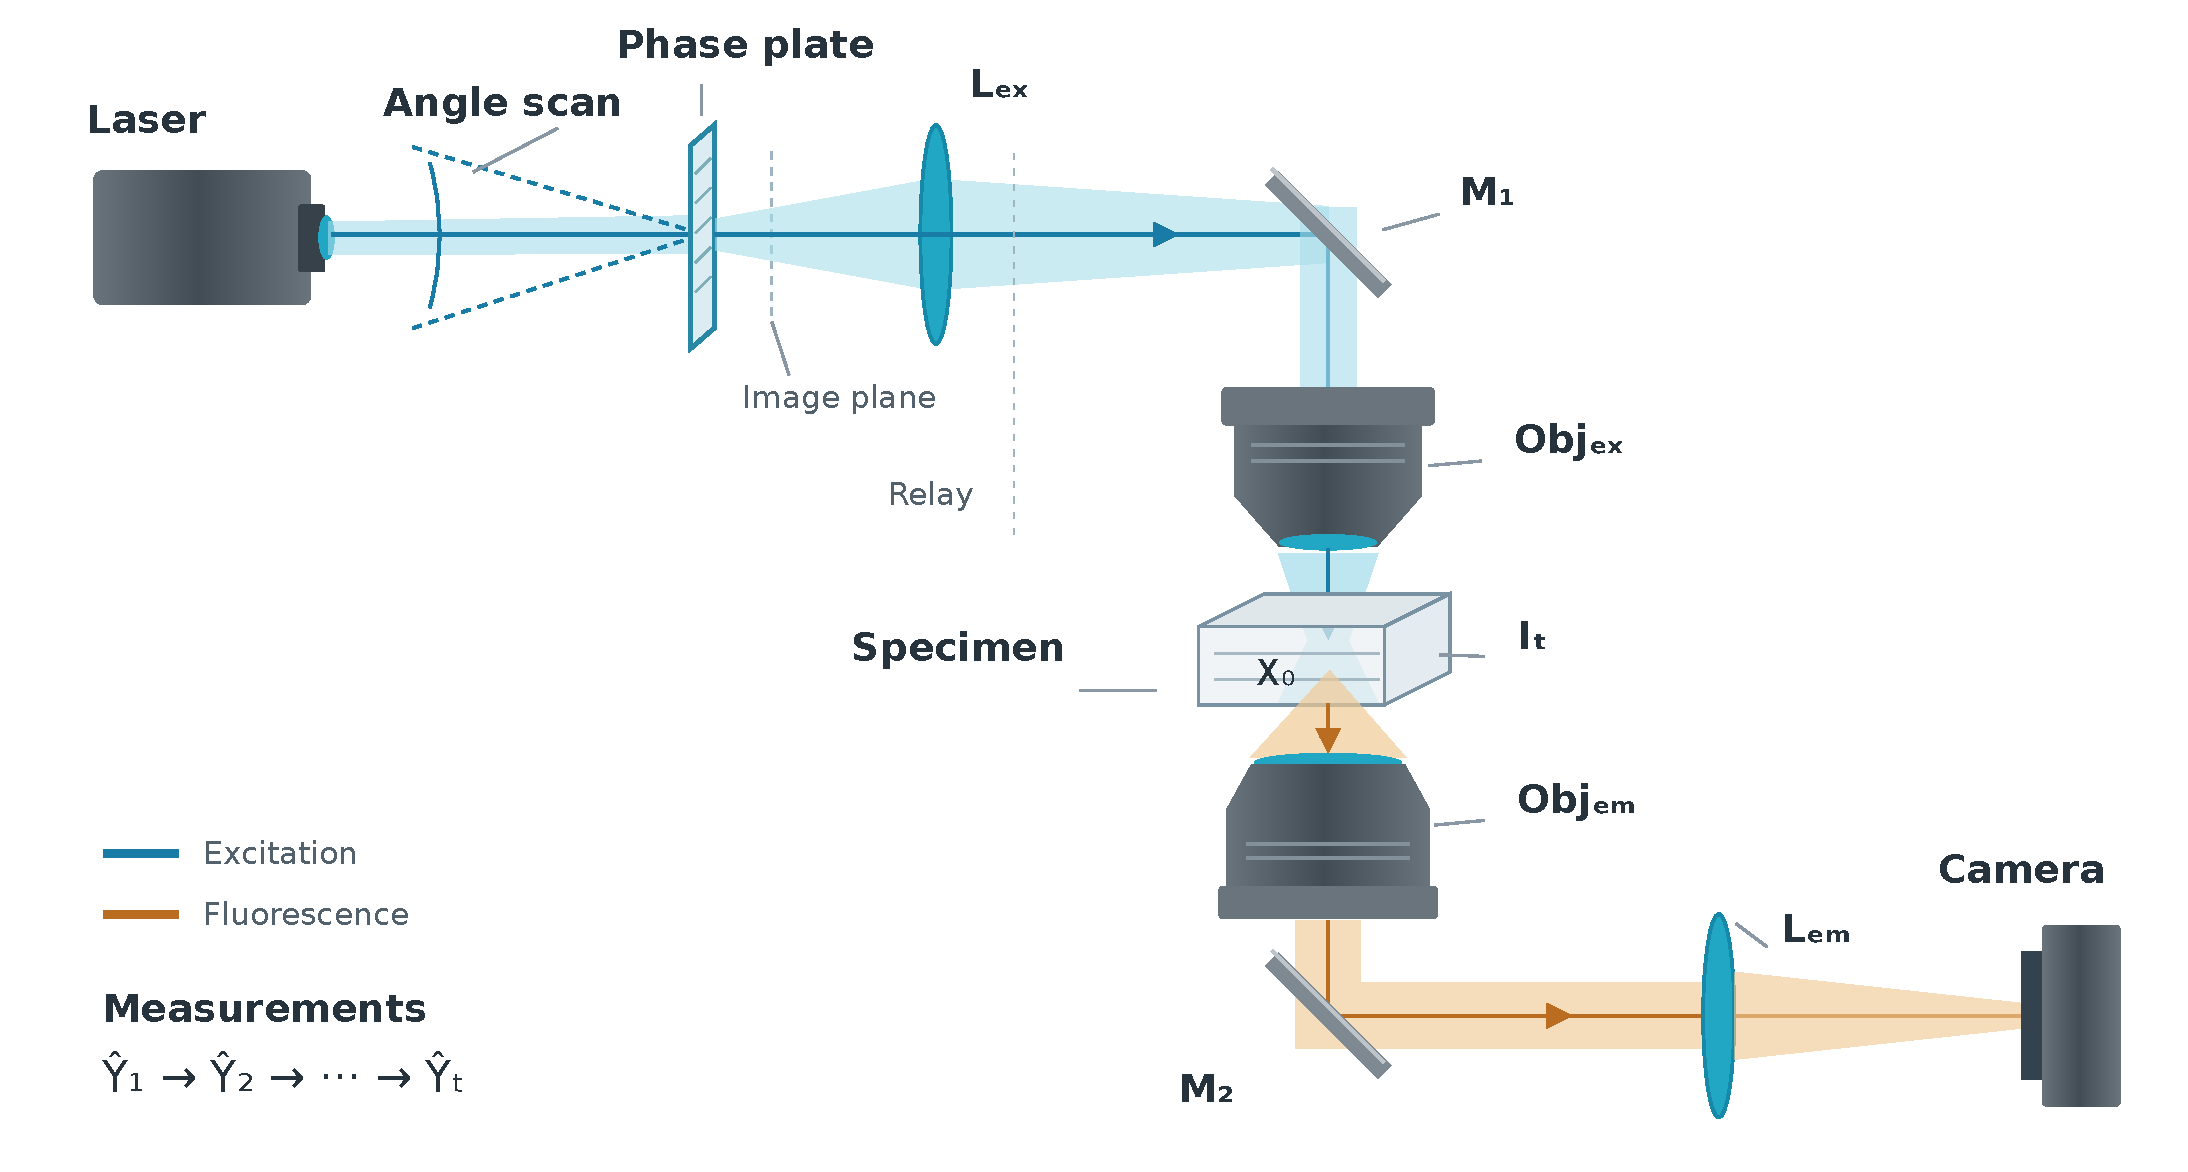
\includegraphics[width=0.90\linewidth,height=0.38\textheight,keepaspectratio]{figures/acquisition.pdf}
\caption{Proposed acquisition. Varying the input angle at a fixed phase encoder generates
depth-dependent illumination while the specimen and detection focus remain fixed.
Blue: excitation; orange: fluorescence.}
\label{fig:acquisition}
\end{figure}


A tilted plane wave illuminates a fixed phase plate defocused from an intermediate illumination image plane. The excitation relay maps the resulting field into the specimen. Changing the incident direction changes the volumetric illumination, while the plate, specimen and detection focus remain fixed.

The plate represents a phase-only encoder. A spatial light modulator (SLM) could display the same phase profile, held fixed during angle variation. Learning a profile or a stack of diffractive layers would instead provide a diffractive deep neural network (D2NN) encoder, a future extension \cite{lin2018}.

Let \(\mathbf r=(x,y)\), and let \(t\) index the illumination direction. The incident field and plate transmission are
\[
u_t^{\mathrm{in}}(\mathbf r)
=a_t e^{\mathrm i k_{\mathrm{ex}}\mathbf s_t\cdot\mathbf r},
\qquad
\tau(\mathbf r)=e^{\mathrm i\phi(\mathbf r)}.
\tag{1}
\]
Here \(a_t\) is the field amplitude, \(k_{\mathrm{ex}}\) the excitation wavenumber and \(\mathbf s_t\) the transverse direction vector. The scan follows directly from plane-wave geometry. With azimuth \(\alpha_t\) and elevation \(\theta_t\) measured from the transverse plane, the propagation direction is \((\cos\theta_t\cos\alpha_t,\cos\theta_t\sin\alpha_t,\sin\theta_t)\). Restricting its phase to the plate plane gives
\[
\mathbf s_t=\cos\theta_t(\cos\alpha_t,\sin\alpha_t),\qquad
\varphi_t(x,y)=k_{\mathrm{ex}}\cos\theta_t
(x\cos\alpha_t+y\sin\alpha_t).
\tag{1a}
\]
Thus the two scan coordinates control the direction and magnitude of the transverse phase gradient. Their sampling determines the sequence of volumetric excitation patterns, rather than changing the detection plane.

Angular-spectrum propagation carries the field through the plate to the relay object plane. High numerical aperture (NA) requires a vectorial description of the transverse and longitudinal field components. The excitation intensity is
\[
I_t^{\mathrm{raw}}(\mathbf r,z)
=\sum_{c\in\{x,y,z\}}|E_{t,c}(\mathbf r,z)|^2.
\tag{2}
\]
We form intensity after field propagation, then average it onto the analysis grid and apply a global scale. The vectorial relay follows the Richards--Wolf formulation and the x-polarised kernel of Marian et al \cite{richards1959,marian2007}.

\subsection{Image formation and reconstruction basis}

\(X_0(\mathbf r,z)\) denotes the fluorescence distribution and \(\mathrm{emPSF}\) the detection intensity point spread function (PSF). Under linear fluorescence,
\[
Y_t=\mathrm{emPSF}*_3(\eta X_0 I_t),
\qquad
\widehat Y^0_{t,p}
=\frac{1}{|D_p|}\int_{D_p}
Y_t(\mathbf r,z_{\mathrm{focal}})\,\mathrm d\mathbf r.
\tag{3}
\]
Here \(*_3\) denotes three-dimensional convolution and \(D_p\) a detector-pixel region. Fluorescence adds incoherently, and the camera samples the same focal plane for every pattern. The fixed factor \(\eta\) is absorbed into the numerical scale. Each pixel value is one scalar measurement \cite{zheng2021,wijethilake2023}.

The multiplication \(X_0 I_t\) explains how fine illumination structure contributes to recovery. It mixes specimen and illumination spatial frequencies before fluorescence is blurred and averaged at the detector, allowing some otherwise unresolved specimen structure to influence measurable intensity variations. The detector need not resolve the illumination pattern itself. As the incident angle changes, locations at different depths experience different illumination sequences. Reconstruction uses these depth-dependent signatures to separate contributions that overlap in individual camera images. Depth separation therefore depends on how the illumination varies across the volume and scan, not on fine spatial structure alone.

Representing this modulation accurately requires different sampling grids for optical simulation and reconstruction. We retain fine-grid optical responses rather than simulate directly at the reconstruction spacing. Let \(\mathsf B\) denote the fine-grid measurement process, and let each reconstruction voxel represent constant fluorescence over a fine-grid patch. With patch replication \(\mathsf U\) and patch averaging \(\mathsf R\), the operator and reference are
\[
\mathsf A=\mathsf B\mathsf U,
\qquad
\mathbf x_{\mathrm{gt}}=\mathsf R\mathbf x_f,
\qquad
\mathbf y=\mathsf B\mathbf x_f+\boldsymbol\varepsilon.
\tag{4}
\]
Thus each operator column integrates the response over a voxel patch. Measurements are generated from the finer object \(\mathbf x_f\), retaining within-patch variation that the reconstruction cannot represent. The remaining representation residual is \(\boldsymbol\delta_{\mathrm{disc}}=\mathsf B(\mathbf x_f-\mathsf U\mathsf R\mathbf x_f)\).

\subsection{Tractable construction of the voxel-integrated operator}

Voxel integration would otherwise require a volumetric simulation for every operator column and illumination pattern. We make the construction tractable by factorising each response into an illumination value and a reusable emission footprint.

For a unit impulse \(\delta_i\) at fine-grid position \(\mathbf r_i=(x_i,y_i,z_i)\), convolution shifts the emission PSF, giving
\[
\begin{aligned}
(\mathsf B_t\delta_i)_p
&=I_t(\mathbf r_i)\,
\mathsf P_p\!\left[\mathrm{emPSF}(\,\cdot-\mathbf r_i)\right]\\
&=I_t(\mathbf r_i)\,g_p(\mathbf r_i).
\end{aligned}
\tag{5a}
\]
Here \(\mathsf P_p\) selects the detection plane and averages over pixel \(p\). The footprint \(g_p\) is independent of illumination and is computed once for all patterns.

Summing over the fine-grid patch \(\mathcal P_j\) of reconstruction voxel \(j\) gives
\[
\mathsf A_{(t,p),j}
=\sum_{i\in\mathcal P_j} I_t(\mathbf r_i)\,g_p(\mathbf r_i).
\tag{5b}
\]
This directly constructs the patch-basis operator \(\mathsf A=\mathsf B\mathsf U\), with the same sampling and padding as the forward model.

For \(T\) patterns, \(P\) detector samples per image, \(N\) reconstruction voxels and \(F\) fine-grid voxels, fast Fourier transform (FFT)-based column simulation and footprint-based assembly cost
\[
C_{\mathrm{column}}=O(TNF\log F),
\qquad
C_{\mathrm{assembly}}=O(TPF).
\tag{5c}
\]
Both expressions exclude shared illumination calculation; assembly also excludes one-time footprint preparation.

The derivation made the volumetric simulation and reconstruction workflow computationally feasible within the available resources. The final operator build, including preparation and validation, takes 109 s on an RTX 4500 Ada GPU.

\subsection{Multi-slice plug-and-play recovery}

\begin{figure}[htbp]
\centering
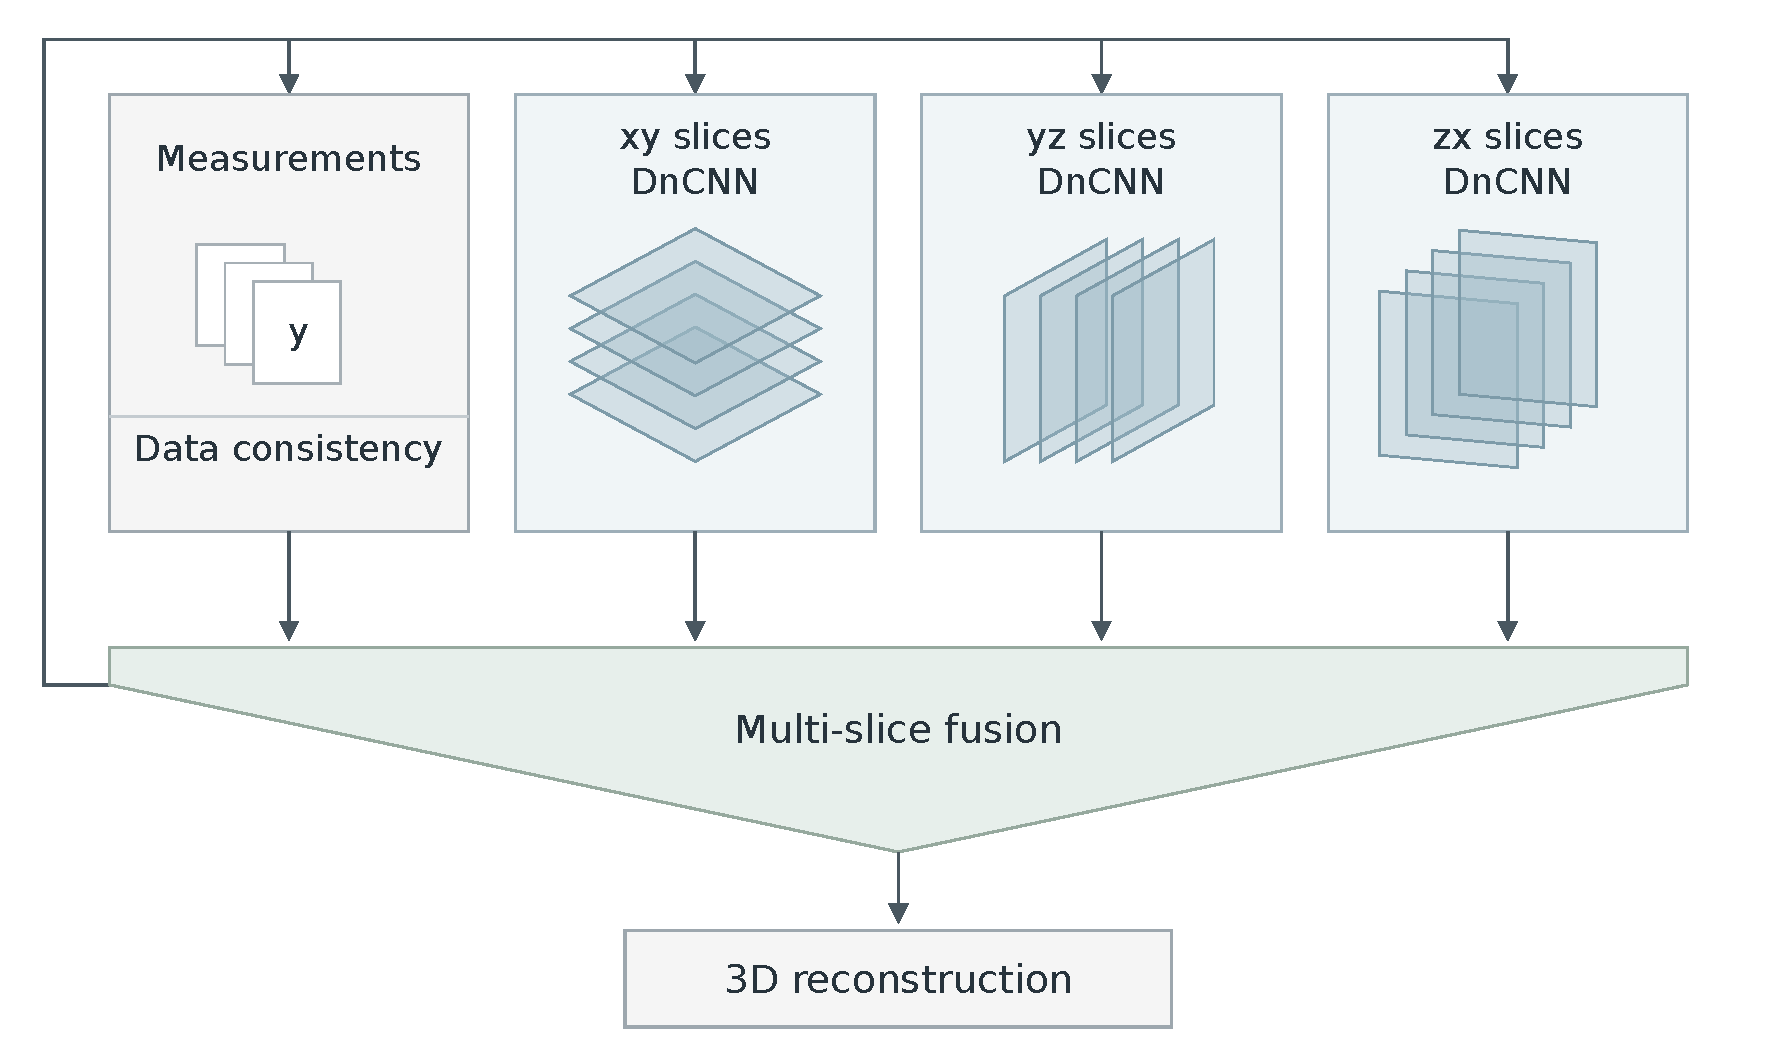
\includegraphics[width=\linewidth,height=0.38\textheight,keepaspectratio]{figures/reconstruction.pdf}
\caption{Multi-slice plug-and-play reconstruction. Measurement consistency and
orthogonal-slice denoising jointly refine a shared volume.}
\label{fig:recovery}
\end{figure}


The planar measurements mix contributions from the volume. We combine measurement consistency with a pretrained two-dimensional denoiser applied to the \(xy\), \(yz\) and \(zx\) slice sets. The same denoiser weights are held fixed across all orientations and throughout reconstruction: no task-specific denoiser or end-to-end reconstruction network is trained. Each orientation views the same volume, and all branches are coupled through a common update. For orientation \(o\), \(\mathcal D_o=\mathsf P_o^{-1}\mathcal D\mathsf P_o\), where \(\mathsf P_o\) arranges the slices and \(\mathcal D\) is the shared denoiser. This follows established PnP and multi-slice fusion principles \cite{venkat2013,majee2021}.

We use the alternating direction method of multipliers (ADMM), with one auxiliary volume \(\mathbf v_j\), dual state \(\mathbf d_j\) and penalty \(\rho_j\) per branch. For \(\mathcal J=\{xy,yz,zx,\mathrm{sp}\}\), including a sparsity branch, the shared update is
\[
\mathbf x^{k+1}=\arg\min_{\mathbf x}
\left\{\frac12\|\mathsf A\mathbf x-\mathbf y\|_2^2+
\sum_{j\in\mathcal J}\frac{\rho_j}{2}
\|\mathbf x-\mathbf v_j^k+\mathbf d_j^k\|_2^2\right\}.
\tag{6}
\]
The quadratic subproblem is solved approximately by conjugate gradients. The branch and dual updates are
\[
\begin{aligned}
\mathbf v_o^{k+1}&=\mathcal D_o(\mathbf x^{k+1}+\mathbf d_o^k),
&&o\in\{xy,yz,zx\},\\
\mathbf v_{\mathrm{sp}}^{k+1}
&=\mathcal S_{\lambda_{\mathrm{sp}}/\rho_{\mathrm{sp}}}
(\mathbf x^{k+1}+\mathbf d_{\mathrm{sp}}^k),\\
\mathbf d_j^{k+1}
&=\mathbf d_j^k+\mathbf x^{k+1}-\mathbf v_j^{k+1}.
\end{aligned}
\tag{7}
\]
\(\mathcal S\) is component-wise soft thresholding, with sparsity weight \(\lambda_{\mathrm{sp}}\). The denoiser acts as an implicit prior, and fusion refines one volume throughout the iterations. We initialise with a normalised backprojection and clip the final estimate to \([0,1]\).
